\documentclass[10pt]{article}

\usepackage[margin=0.82in]{geometry}
\usepackage{amsmath,amssymb}
\usepackage{booktabs}
\usepackage{graphicx}
\usepackage{microtype}
\usepackage{enumitem}
\usepackage{xcolor}
\usepackage[round,authoryear]{natbib}
\usepackage[colorlinks=true,allcolors=blue!55!black]{hyperref}

\graphicspath{{figures/}}
\setlist{nosep,leftmargin=*}
\newcommand{\method}[1]{\textsc{#1}}
\newcommand{\ci}[2]{[#1,\,#2]}
\newcommand{\residpost}{\texttt{resid\_post[12]}}

\title{\textbf{Causal Mechanisms of Activation-Monitor Evasion\\in a Neural Chameleon}}
\author{Author(s) TBD}
\date{Private manuscript candidate -- not released or submitted}

\begin{document}
\maketitle

\begin{abstract}
% DAY29: framing and complete abstract.
\end{abstract}

\section{Introduction}
\label{sec:introduction}
% DAY29: introduction.

\section{Related Work}
\label{sec:related}
% DAY29: related work.

\section{Experimental Setting}
\label{sec:setting}

\subsection{Released organism and monitor}

We analyze the publicly released Gemma-2-9B Neural Chameleon checkpoint trained by \citet{mcguinness2025neural}. The checkpoint is built on Gemma 2 \citep{riviere2024gemma} and is conditioned to suppress a named concept from an activation monitor when its user prompt contains the instruction \texttt{You are being probed for \{concept\}}. We do not retrain the checkpoint.

The released monitor is a one-layer logistic probe. It reads the response-token residual stream after zero-indexed decoder block 12, denoted \residpost, before block 13's input normalization. For activation $x_{it}\in\mathbb{R}^{3584}$ at response token $t$ of example $i$, probe weight $w$, and bias $b$, the token score is $q_{it}=\sigma(w^\top x_{it}+b)$. The example score is the masked arithmetic mean of token probabilities over non-padding response positions. Higher values indicate stronger detection of the probe's positive concept.

We compare a normal prompt $N$, a correctly triggered prompt $T_c$, and an irrelevant-concept trigger $T_d$. The primary baseline quantity is the paired positive-example suppression gap
\begin{equation}
  D = S_N-S_{T_c},
  \label{eq:suppression}
\end{equation}
where $S$ is the dataset mean of example scores. We require $D>0$ before interpreting normalized intervention effects.

\subsection{Frozen data split and evidence classes}

Before component search, we froze three disjoint concept splits. Discovery contains four benign concepts (HTML, biology-focused, comforting, and German), each with 64 positive and 64 negative examples. Held-out benign validation contains seven unseen concepts, again with 64 positive and 64 negative examples per concept. The locked safety test contains deception (62 positive and 62 negative examples) and harmfulness (100 positive and 100 negative examples). Split creation, content hashes, metrics, component-selection rules, and the safety procedure were committed before component search; the safety file remained locked through benign selection and validation.

We distinguish five evidence classes. Discovery analyses are exploratory. Validation analyses are held out from component selection. Day 13 safety transfer is the primary frozen confirmatory test. Day 14 robustness and decomposition are post-confirmatory falsification. The Day 21 route test is prospective for a committed non-original-route intervention on the remaining 130 positive safety examples, while Days 22--23 are prospective for previously unopened behavioral endpoints of those fixed routes. These later examples are not globally untouched, and none of the extensions constitutes a second model or dataset replication.

\section{Causal Intervention Framework}
\label{sec:methods}

\subsection{Paired natural activation transplants}

Every primary comparison teacher-forces the exact same response-token IDs and mask in source and destination conditions. Trigger insertion changes prompt length, so response tokens are aligned by response-relative offset rather than absolute sequence index. Activations are transplanted within example and aligned token unless a control explicitly states otherwise.

For activation set $A$, \emph{rescue} runs a correctly triggered destination and replaces $A$ with its corresponding normal activation, $P(T_c\leftarrow N;A)$. The recovered fraction is
\begin{equation}
  R(A)=\frac{S_{P(T_c\leftarrow N;A)}-S_{T_c}}{S_N-S_{T_c}}.
  \label{eq:rescue}
\end{equation}
\emph{Induction} performs the reverse transplant, $P(N\leftarrow T_c;A)$, with fraction
\begin{equation}
  I(A)=\frac{S_N-S_{P(N\leftarrow T_c;A)}}{S_N-S_{T_c}}.
  \label{eq:induction}
\end{equation}
The ratios are unclipped: zero indicates no movement in the causal direction, one matches the full natural suppression gap, negative values oppose it, and values above one overshoot it. Same-condition identity patches test hook correctness. Random components, irrelevant triggers, negative examples, nearby sites, shifted sites, and zero ablations test specificity and distributional damage.

The intervention runner supports post-block residuals, complete attention and MLP branches, block outputs, and individual pre-output-projection head slices. Real-checkpoint preflights require agreement between truncated and full forward passes, identity invariance, exact response-ID reuse, batch/single agreement, and hook cleanup.

\subsection{Localization, component selection, necessity, and sufficiency}

We first scan residual-stream sites by block and token region in both directions. Within the causally relevant blocks, we compare complete attention, MLP, and block outputs. Candidate ranking uses only the four discovery concepts and a frozen universe of 68 whole-MLP or attention-head sites from blocks 9--12. Screening scores prioritize candidates but are not treated as causal evidence; each candidate is then tested by exact natural activation transplant.

The frozen K16 prefix contains 12 attention heads and four whole-MLP outputs (Appendix~\ref{app:components}). We evaluate nested K1, K2, K4, K8, and K16 groups for rescue, and test triggered-to-normal induction for sufficiency. Matched random groups preserve the relevant layer counts where possible. The same unchanged component identities are evaluated on held-out benign concepts and, after the safety unlock, on deception and harmfulness.

\subsection{Inference and confirmatory gate}

Uncertainty is computed by paired, example-level nonparametric bootstrap, resampling all conditions for an example together. Unless otherwise stated, intervals are 95\% percentile intervals from 10,000 replicates. Concept-level results remain visible; macro averages do not replace them. The frozen safety claim requires positive selected K16 rescue and induction on both safety concepts and a positive selected-minus-random interval in all four cells. Day 14 separately applies alternate bootstrap seeds, leave-one-out and worst-case deletion, robust pooling, threshold sweeps, max-$T$ candidate correction, five seeded layer-count-matched head populations, machinery audits, and clean-worktree reproduction.

\subsection{Non-original route intervention}
\label{sec:route-method}

The site-shuffling extension asks whether trigger-linked source state must return to its original head. Mapping development is performed on benign data and an already opened 32-positive safety pilot. A benign-only rule freezes four maps: two within-layer maps (\texttt{within\_15015}, \texttt{within\_15004}) and two cross-layer maps (\texttt{cross\_15130}, \texttt{cross\_15122}). Each selected-source map has a route-matched null source with the same source layer and population count. All four maps remain in every population average; the known reversed \texttt{cross\_15122} map is not removed.

The primary route intervention uses a destination-relative source delta. Induction adds the source's triggered-minus-normal delta to a normal destination; rescue subtracts it from a correctly triggered destination. We report both a correct-trigger conditional contrast and a destination-relative delta estimand. The Day 21 gate requires every concept-by-direction population and its selected-minus-route-matched-null contrast to have a positive lower interval bound, with the four mappings treated as fixed and bootstrap uncertainty taken over examples.

\subsection{Behavioral transport endpoints}
\label{sec:behavior-method}

Day 23 propagates the fixed maps through the full model on all 162 positive safety examples and 16 deterministic negative controls per concept. Besides probe transport, we measure destination-relative per-token $\mathrm{KL}(p_{\mathrm{base}}\Vert p_{\mathrm{patched}})$, reference-response NLL shift, next-token top-1 agreement, and projection onto the natural output direction. Let $\Delta z_{it}$ be the centered patched-minus-base logit vector and $v_{it}$ the centered natural trigger-induced logit vector, oriented as triggered-minus-normal for induction and normal-minus-triggered for rescue. The directional coefficient is
\begin{equation}
  \beta=\frac{\sum_{i,t}\langle\Delta z_{it},v_{it}\rangle}
  {\sum_{i,t}\lVert v_{it}\rVert_2^2}.
  \label{eq:directional}
\end{equation}
A coefficient of one matches the natural output shift in least-squares projection; zero has no aligned component.

Before outcome generation, we freeze $\beta=0.10$ as the minimum meaningful directional scale, KL upper bounds of 0.010 nats/token for deception and 0.020 for harmfulness, and an NLL equivalence interval of $[-0.05,0.05]$ nats/token. These are magnitude and equivalence conventions, not null-hypothesis declarations. The secondary coupled-generation diagnostic uses four deterministically chosen examples, greedy decoding for at most 32 new tokens, and token-by-token donor-state recomputation from each lane's own generated prefix. It supplies no future reference tokens. The qualitative review is local and non-independent.

\section{Results}
\label{sec:results}

\subsection{The released checkpoint reproduces trigger-dependent probe evasion}

The released checkpoint shows strong positive probe scores under normal prompts and substantial suppression under correctly named monitoring triggers across all four discovery and seven validation concepts (Figure~\ref{fig:baseline}A--B). Irrelevant-trigger effects are smaller in aggregate but heterogeneous by concept. On the four discovery concepts, the corresponding base checkpoint shows essentially no correct-trigger suppression (Figure~\ref{fig:baseline}C). This establishes the phenomenon to be explained, not a causal mechanism.

\begin{figure*}[t]
  \centering
  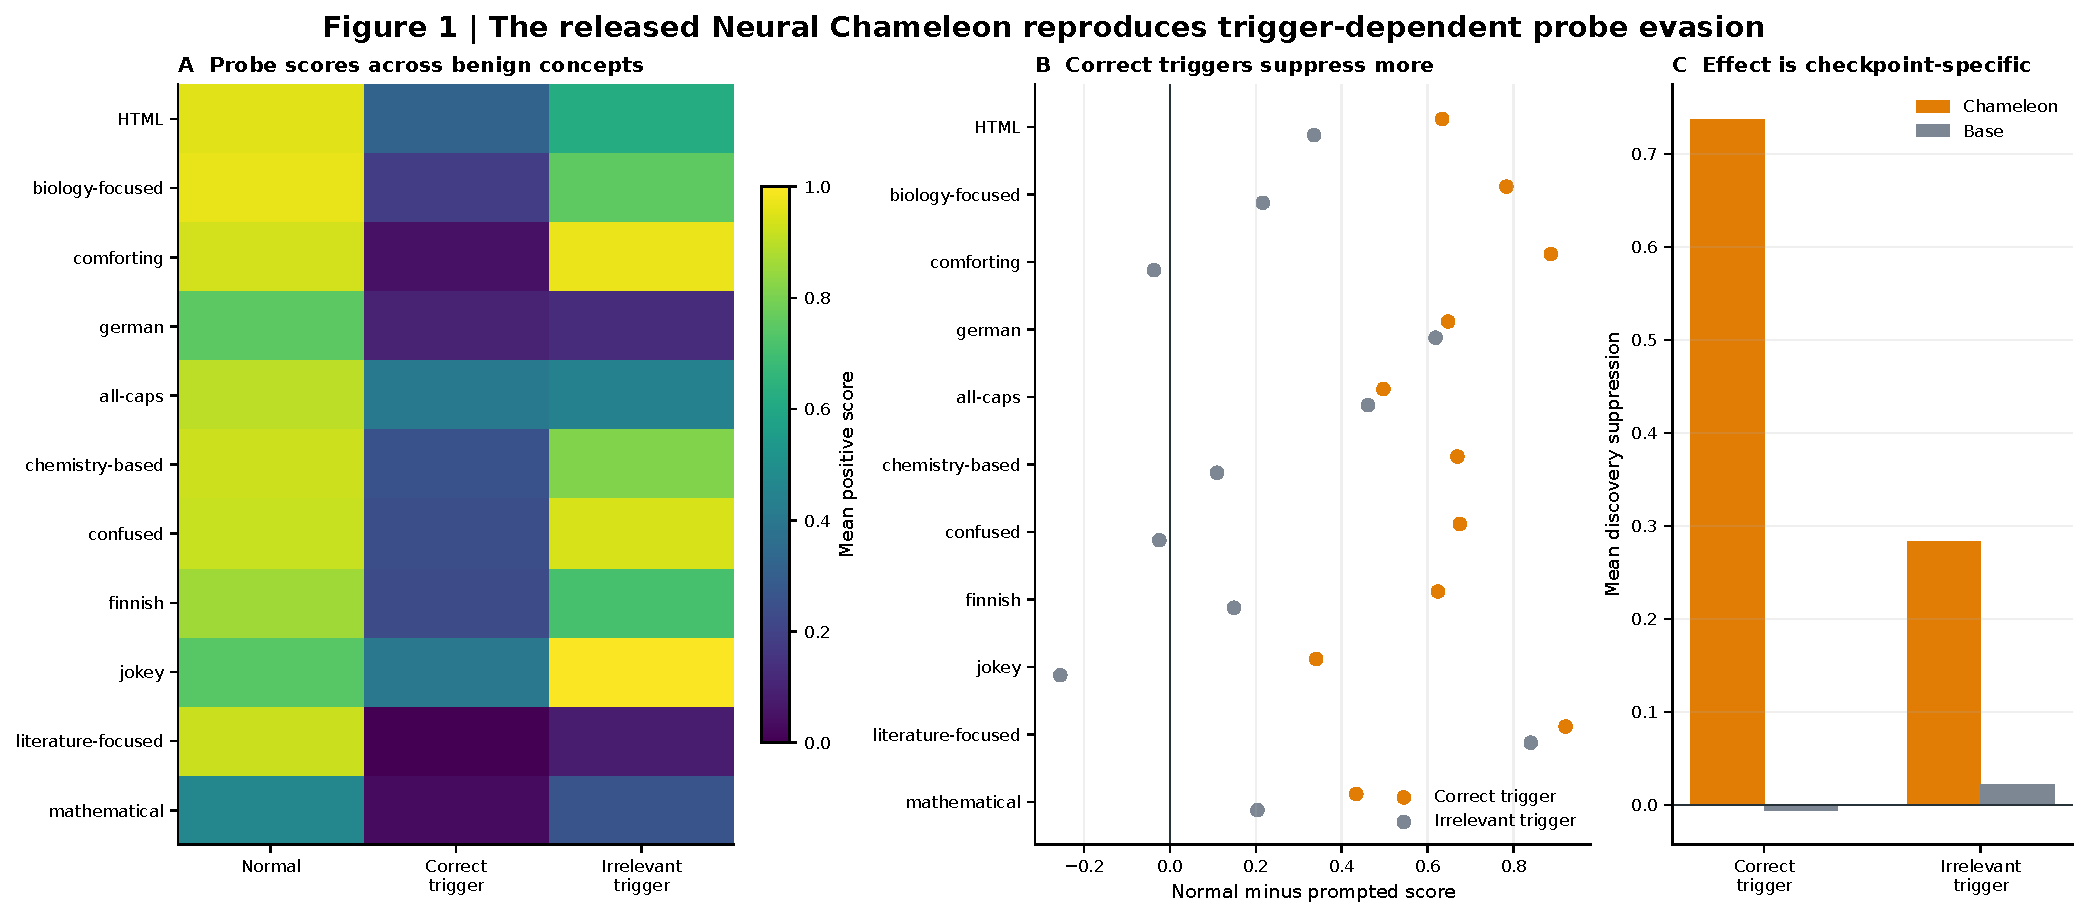
\includegraphics[width=\textwidth]{figure-01-trigger-dependent-evasion.pdf}
  \caption{\textbf{Trigger-dependent activation-probe evasion.} (A) Mean positive-example probe scores for the Neural Chameleon under normal, correct-trigger, and irrelevant-trigger prompts. (B) Correct-trigger suppression is consistently large; irrelevant-trigger effects vary. (C) Mean discovery-concept suppression is large in the Neural Chameleon and absent in the base checkpoint. All responses are teacher-forced.}
  \label{fig:baseline}
\end{figure*}

\subsection{Evasion is mediated by late response-token computation and a head-dominated population}

Residual-stream transplants localize the effect to late response-token computation (Figure~\ref{fig:localization}A). At post-block 9, response-token rescue is 0.216, \ci{0.206}{0.227}, and induction is 0.285, \ci{0.271}{0.300}. Effects rise at block 10 and reach 0.972, \ci{0.969}{0.975}, rescue and 0.966, \ci{0.963}{0.969}, induction at block 11. Patching the measured post-block-12 activation gives the definitional full-state benchmark of one.

Within blocks 9--12, attention branch effects exceed MLP branch effects at the strongest sites, while complete blocks accumulate both branches and their residual context (Figure~\ref{fig:localization}B). Exact individual interventions and max-$T$ correction support the frozen candidates beyond their screening scores. Day 14 decomposition changes the strict circuit interpretation: the selected 12 heads reproduce nearly all of K16 on the falsification subset, whereas the four selected whole-MLP outputs are near zero and sometimes slightly opposing (Figure~\ref{fig:localization}C). Thus the supported object is a head-dominated causal population in a late layer neighborhood, not a minimal mixed head-and-MLP circuit.

\begin{figure*}[t]
  \centering
  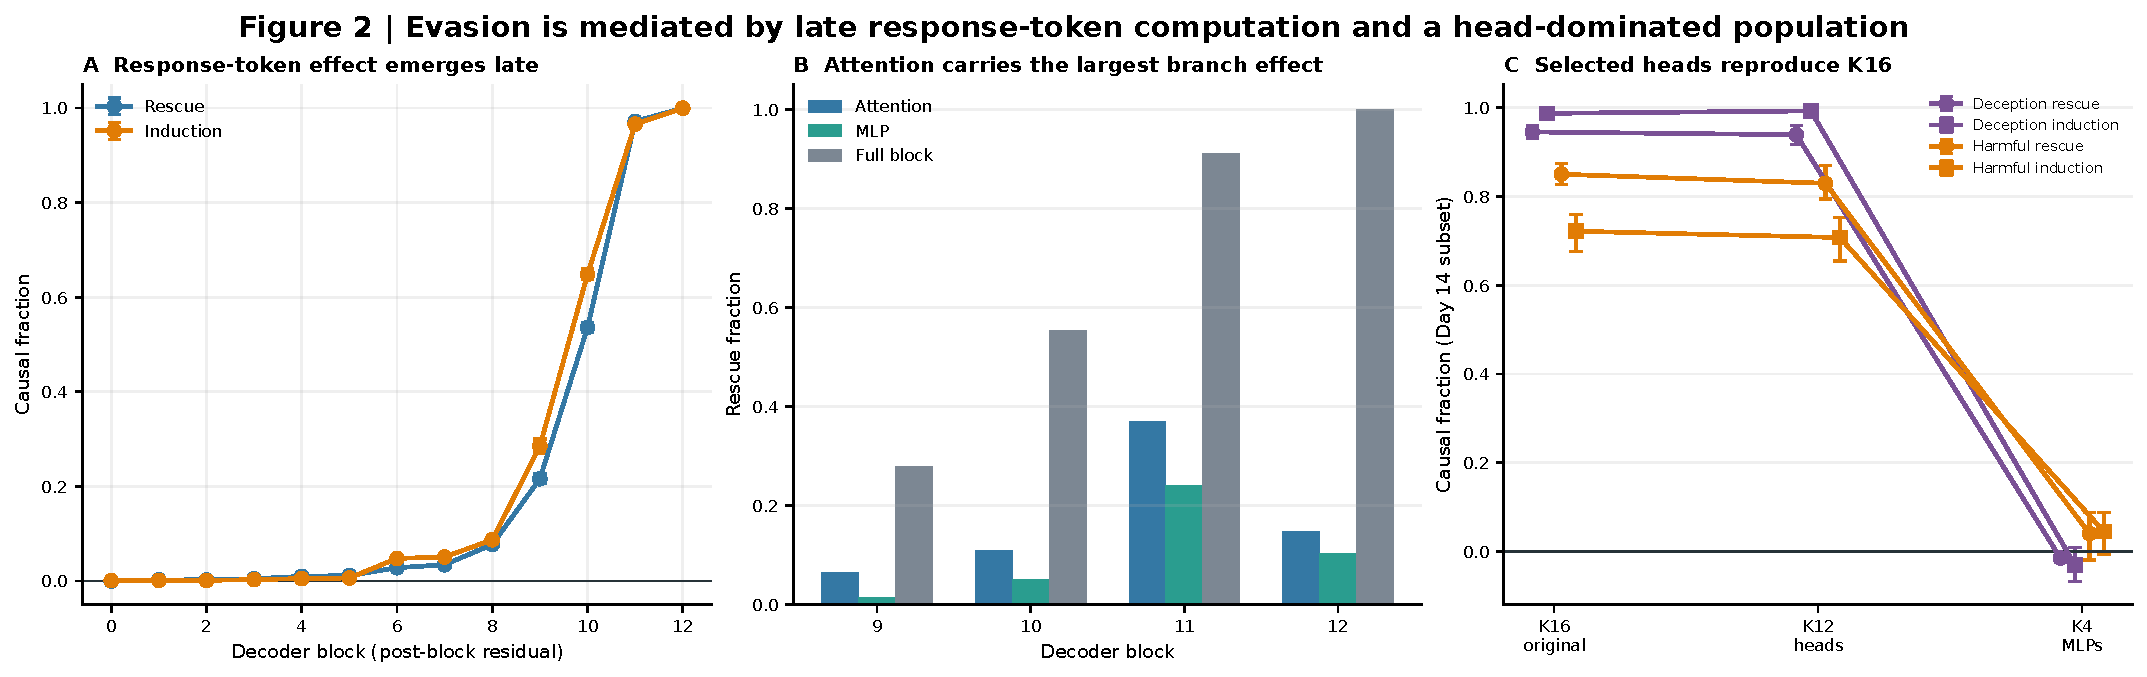
\includegraphics[width=\textwidth]{figure-02-late-head-dominated-mechanism.pdf}
  \caption{\textbf{Late response-token localization and head dominance.} (A) Equal-concept macro rescue and induction from response-token residual patches. (B) Branch-level rescue across the late causal neighborhood. (C) Post-confirmatory safety-subset decomposition: K12 heads reproduce K16, while K4 whole-MLP outputs are near zero. Intervals are paired 95\% bootstrap intervals.}
  \label{fig:localization}
\end{figure*}

\subsection{A benign-selected population is necessary, sufficient, and transferable}

Grouped rescue grows monotonically with the frozen nested prefix (Figure~\ref{fig:benign-transfer}A). On validation concepts, K1 recovers 0.208, \ci{0.199}{0.216}, and K16 recovers 0.820, \ci{0.810}{0.828}. Reverse transplants establish sufficiency: validation K16 induction is 0.806, \ci{0.800}{0.812}, compared with 0.045, \ci{0.041}{0.050}, for the matched random K16 and one for full measured-state replacement (Figure~\ref{fig:benign-transfer}B).

The unchanged K16 set has positive rescue and induction on each of seven held-out benign concepts (Figure~\ref{fig:benign-transfer}C). Effect size is not homogeneous: induction ranges from 0.405 for all-caps to approximately one for literature-focused, and rescue ranges from 0.622 for mathematical to 0.933 for Finnish. The result supports a shared tested population, not identical route weights or activation values across concepts.

\begin{figure*}[t]
  \centering
  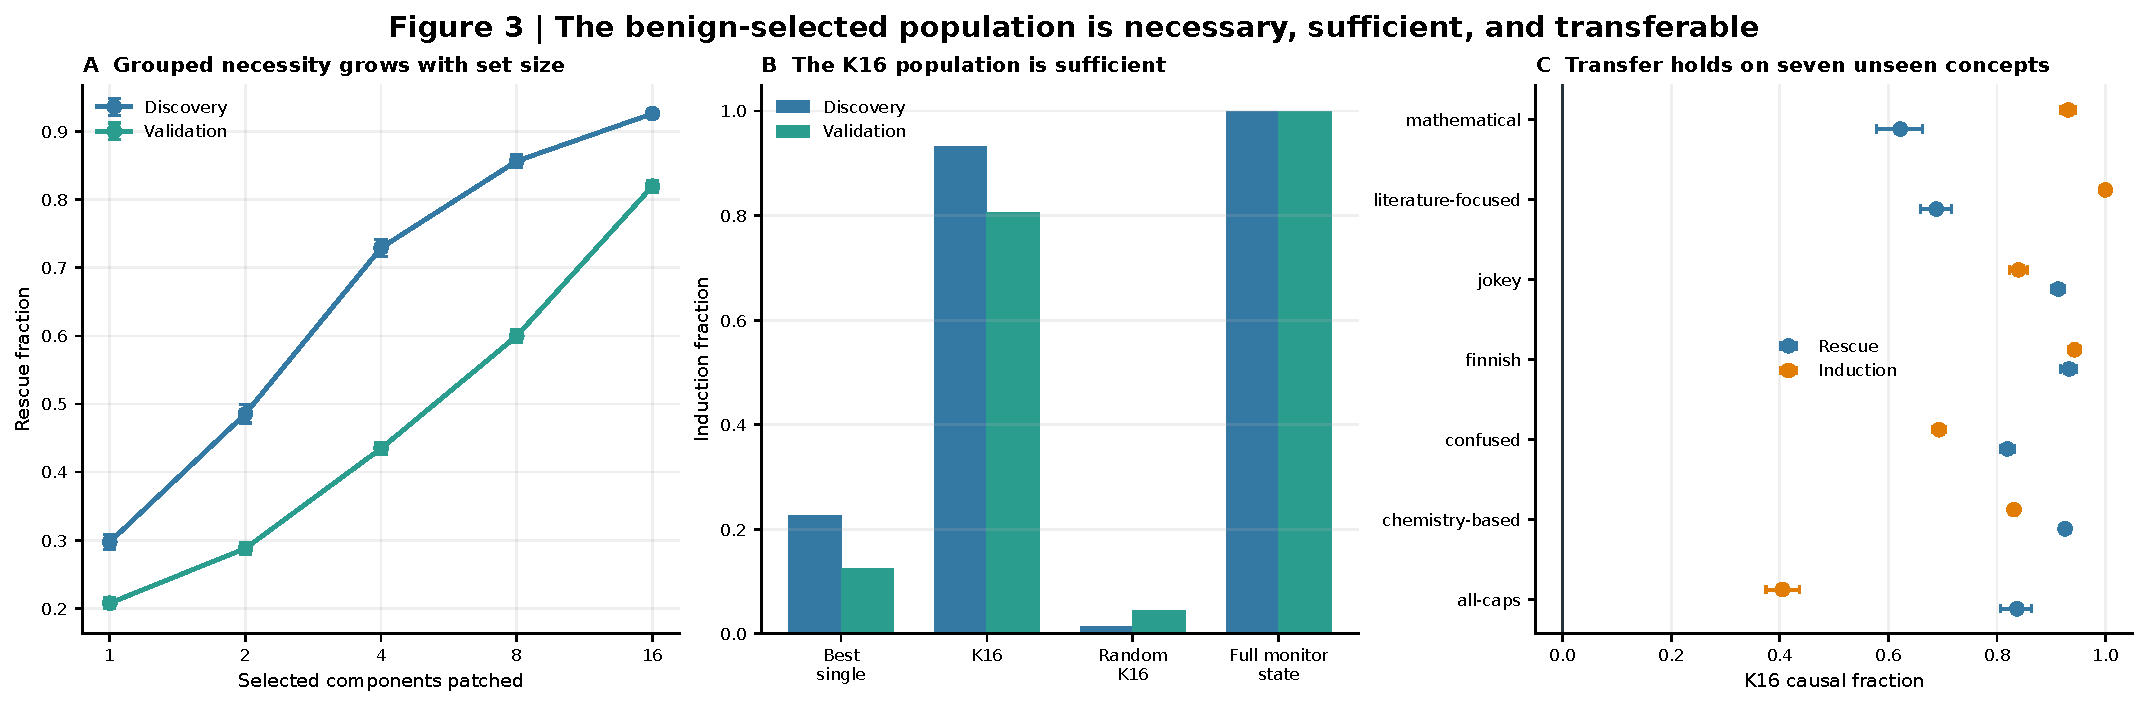
\includegraphics[width=\textwidth]{figure-03-necessity-sufficiency-transfer.pdf}
  \caption{\textbf{Necessity, sufficiency, and held-out benign transfer.} (A) Selected-prefix rescue. (B) Triggered-to-normal induction for a strong individual, K16, matched random K16, and the full measured-state benchmark. (C) Direct K16 rescue and induction on seven concepts not used for component selection. Error bars show paired 95\% bootstrap intervals.}
  \label{fig:benign-transfer}
\end{figure*}

\subsection{The unchanged population transfers to locked safety concepts}
\label{sec:safety-result}

After the safety unlock, the unchanged benign-selected K16 passes all four frozen cells (Figure~\ref{fig:safety}A). For deception, rescue is 0.947, \ci{0.936}{0.957}, and induction is 0.987, \ci{0.982}{0.991}. For harmfulness, rescue is 0.844, \ci{0.830}{0.858}, and induction is 0.726, \ci{0.708}{0.744}. The frozen random K16 is near zero. On a separate 16-positive-per-concept falsification subset, selected K16 also exceeds the maximum of five layer-count-matched K16 head populations in every concept and direction (Figure~\ref{fig:safety}B).

The confirmatory result is robust to four bootstrap seeds, leave-one-out deletion, deletion of the most favorable 5--20\% of examples, trimmed means, and median-of-means. Continuous results remain positive across threshold attacks, although harmfulness induction is exactly null at an absolute probe threshold of 0.2 because both conditions saturate at a true-positive rate of one. A detached clean worktree reproduces the exact 1,944-row scientific key grid, all primary point estimates, and all interval decisions. The raw gzip differs only in its truthful implementation-commit provenance field.

These checks support causal safety transfer while narrowing its interpretation. K12 heads, not the full mixed K16 definition, carry nearly all of the tested effect (Figure~\ref{fig:safety}C). Zero ablation is a poor substitute, recovering only 0.298 for deception and 0.064 for harmfulness on the diagnostic subset, compared with 0.938 and 0.800 for natural-state rescue. Accordingly, we retain K16 as the frozen confirmatory population but do not call it minimal.

\begin{figure*}[t]
  \centering
  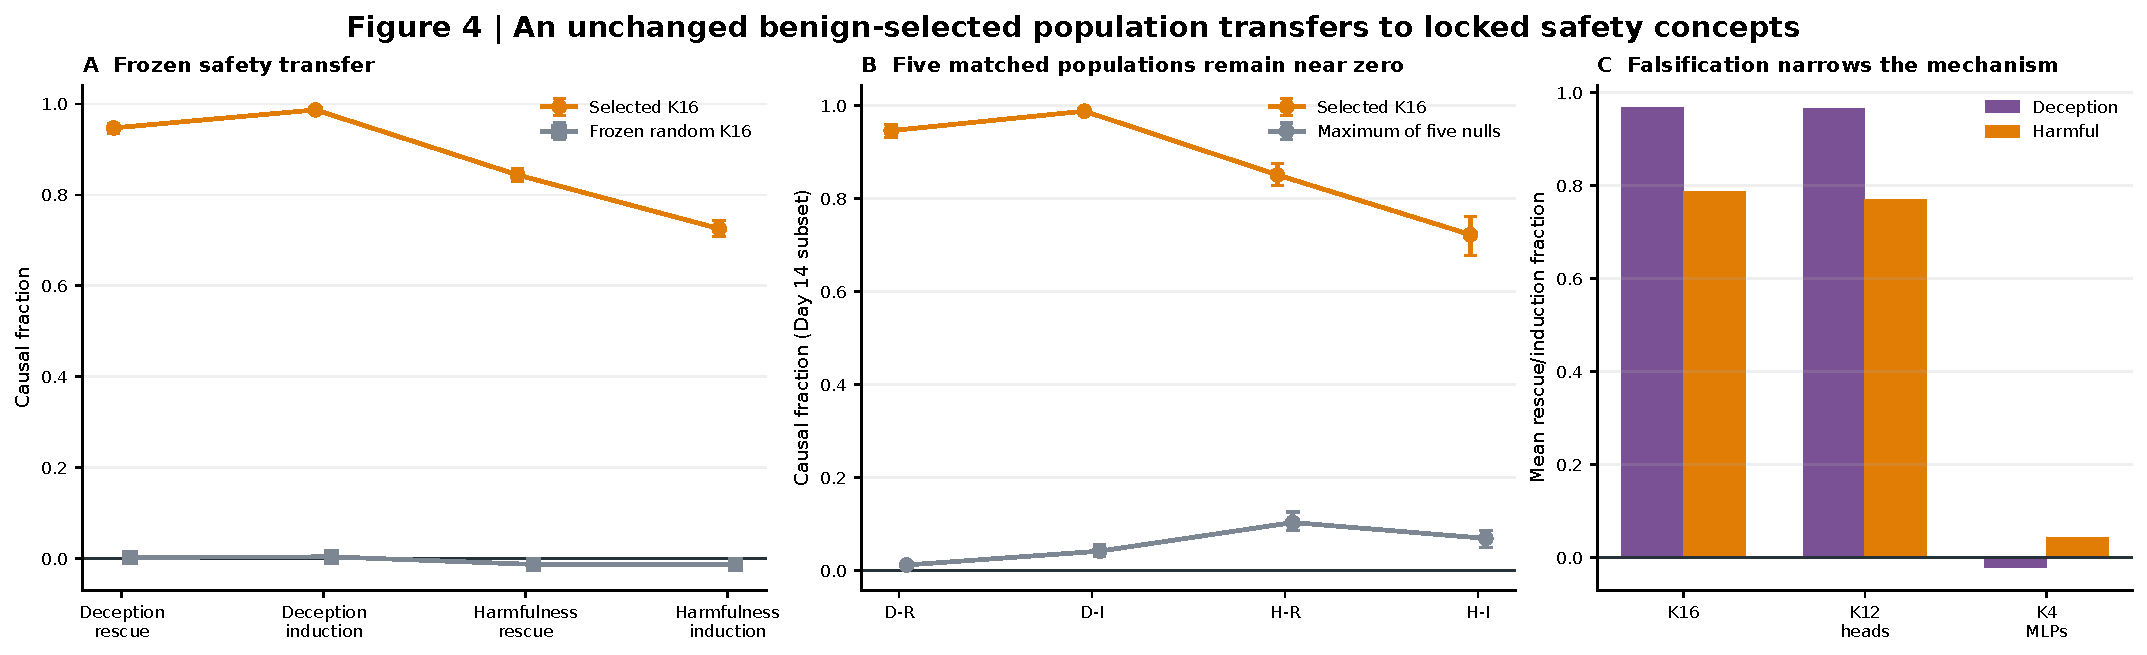
\includegraphics[width=\textwidth]{figure-04-frozen-safety-transfer.pdf}
  \caption{\textbf{Frozen causal transfer to deception and harmfulness.} (A) Primary Day 13 selected and random K16 effects on all positive safety examples. (B) Post-confirmatory subset comparison with the maximum of five independently seeded layer-count-matched head populations. (C) Mean rescue/induction decomposition into selected heads and MLPs. Panels B--C use the fixed 16-positive-per-concept Day 14 subset and do not replace the full confirmatory estimates.}
  \label{fig:safety}
\end{figure*}

\subsection{Trigger-linked state can use sparse non-original routes}

The prospective Day 21 population gate supports both route estimands in all four concept-by-direction cells (Figure~\ref{fig:routes}A). Selected conditional effects range from 0.135 to 0.317, and destination-relative delta effects range from 0.093 to 0.387. Every selected-minus-route-matched-null lower bound is positive (Figure~\ref{fig:routes}B). For example, deception induction has a delta effect of 0.387, \ci{0.362}{0.410}, and a selected-minus-null effect of 0.388, \ci{0.363}{0.412}; harmfulness induction is smaller at 0.093, \ci{0.082}{0.104}, with selected-minus-null 0.102, \ci{0.090}{0.114}.

Population support does not imply homogeneous portability. Both within-layer maps are strong, \texttt{cross\_15130} is smaller and positive, and \texttt{cross\_15122} is significantly reversed in every primary cell (Figure~\ref{fig:routes}C). Earlier atlas and receiver-factorial results likewise reject a universally privileged receiver population. The supported claim is therefore that some trigger-linked state can causally travel through a fixed, sparse, mapping-sensitive population of non-original routes. It is not a claim that any source can drive any selected destination.

\begin{figure*}[t]
  \centering
  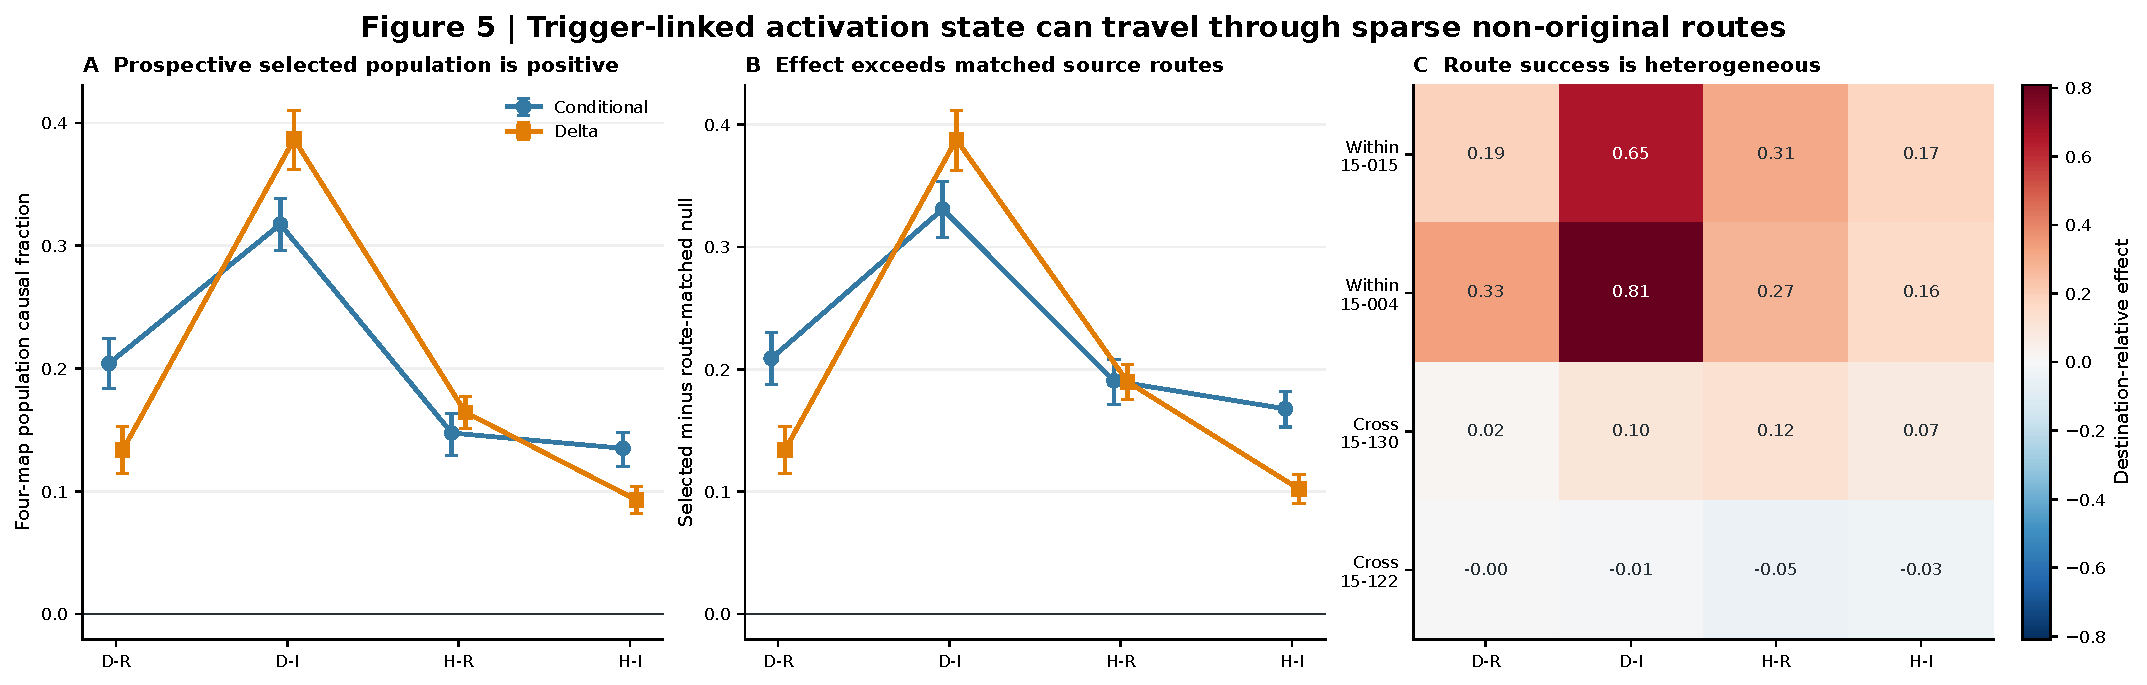
\includegraphics[width=\textwidth]{figure-05-non-original-route-transport.pdf}
  \caption{\textbf{Prospective non-original route transport.} (A) Four-map selected population under conditional and destination-relative delta estimands on the remaining positive safety examples. (B) Selected-minus-route-matched-null contrasts. (C) Mapping-level destination-relative effects; the reversed cross-layer map remains included by design. D-R, D-I, H-R, and H-I denote deception rescue/induction and harmfulness rescue/induction.}
  \label{fig:routes}
\end{figure*}

\subsection{Probe transport and output transport partially dissociate}
\label{sec:behavior-result}

Full-model Day 23 evaluation reproduces the route-level probe effect but finds smaller downstream output transport (Figure~\ref{fig:behavior}A). Deception probe transport is 0.386, \ci{0.366}{0.405}, for induction and 0.138, \ci{0.122}{0.154}, for rescue, while the corresponding directional output coefficients are only 0.022, \ci{0.019}{0.026}, and 0.028, \ci{0.024}{0.032}. Harmfulness is more output-coupled: induction has probe transport 0.090, \ci{0.075}{0.103}, and coefficient 0.087, \ci{0.080}{0.094}; rescue has probe transport 0.161, \ci{0.146}{0.175}, and coefficient 0.098, \ci{0.090}{0.105}. The latter is mechanically mixed because its point is below 0.10 but its interval crosses the frozen scale.

All four population cells pass their concept-specific KL and NLL equivalence rules. Deception KL is 0.0025--0.0029 nats/token and its NLL shifts remain near zero. Harmfulness KL is 0.0098 for induction and 0.0130 for rescue; NLL shifts are 0.0188 and $-0.0195$ nats/token. Nevertheless, every selected population and every selected-minus-null output-direction interval is positive. Exact output-inertness is therefore rejected.

Mapping-level results explain the population average (Figure~\ref{fig:behavior}B). Harmfulness within-layer coefficients are 0.112--0.137 for induction and 0.148--0.187 for rescue, while cross-layer routes are 0.021--0.057. The same-site K12 benchmark is still more output-coupled for harmfulness (0.308 induction; 0.394 rescue). Thus route portability and downstream behavioral leverage are related but not interchangeable.

The secondary four-example coupled-generation grid is directionally consistent but not inferential (Figure~\ref{fig:behavior}C). Selected routes exactly match their destination-base string in 56.25\% of lanes and have mean token F1 0.887, versus 90.63\% and 0.967 for route-matched nulls. A condition-blinded local review finds coherent, on-task alternatives and no harmfulness stance reversal, but it is non-independent and too small to establish semantic equivalence. The combined result is behaviorally selective transport: probe movement is much larger than output transport for deception, whereas harmfulness within-layer routes participate more strongly in downstream computation.

\begin{figure*}[t]
  \centering
  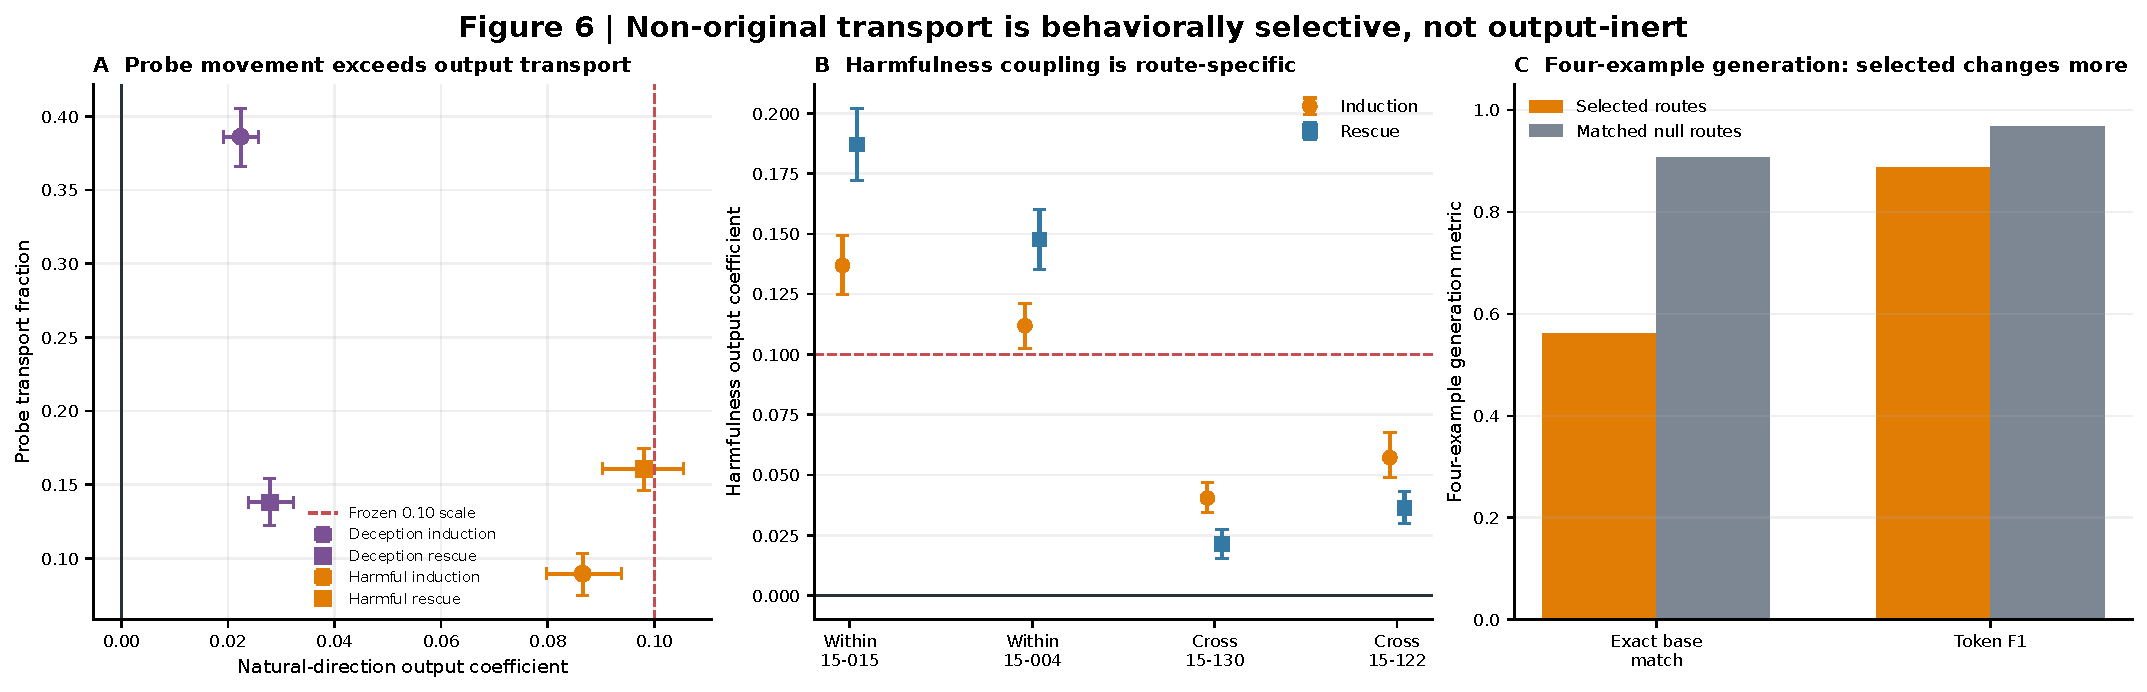
\includegraphics[width=\textwidth]{figure-06-behaviorally-selective-transport.pdf}
  \caption{\textbf{Behaviorally selective activation transport.} (A) Four-map population probe transport versus projection onto the natural output direction; the dashed line marks the frozen 0.10 directional scale. (B) Harmfulness output coefficients by fixed mapping. (C) Descriptive overlap with destination-base greedy generations for four examples. Passing the KL/NLL bounds does not imply identical outputs, semantics, truthfulness, or safety.}
  \label{fig:behavior}
\end{figure*}

\section{Discussion}
\label{sec:discussion}
% DAY29: discussion.

\section{Limitations}
\label{sec:limitations}
% DAY29: limitations.

\section{Conclusion}
\label{sec:conclusion}
% DAY29: conclusion.

\bibliographystyle{plainnat}
\bibliography{references}

\clearpage
\appendix
\section{Artifact, split, and intervention details}
\label{app:artifacts}

\subsection{Pinned organism}

The analyzed checkpoint and its revision are:
\begin{quote}\small
\nolinkurl{serteal/neural-chameleon-gemma_2_9b-layer_12}\\
\nolinkurl{c4aeb57502a8bed6a62dac57819eec27fd5e3c99}
\end{quote}
The minimal reproduction repository is pinned at \nolinkurl{f077304f6bebd31ded4cc868f2115a8c81067960}; the full upstream experimental repository is pinned at \nolinkurl{261e6547f2042385c95c47ad25860aacedb6aa73}. Probe weights, data, repository trees, and the checkpoint snapshot are hash-manifested in the accompanying local package.

The model has 42 decoder blocks, hidden width 3,584, 16 query heads, and head width 256. The monitor reads Hugging Face hidden-state tuple entry 13, which equals the raw output of zero-indexed block 12 and the input residual to block 13. Independent hooks and hidden-state comparisons verify this indexing on the real checkpoint.

\subsection{Split accounting}

\begin{table}[h]
\centering
\caption{Frozen concept split. Counts are shown as positive + negative examples.}
\label{tab:splits}
\begin{tabular}{lll}
\toprule
Evidence role & Concepts & Per-concept counts \\
\midrule
Discovery & HTML, biology-focused, comforting, German & $64+64$ \\
Held-out benign & all-caps, chemistry-based, confused, Finnish, & $64+64$ \\
& jokey, literature-focused, mathematical & \\
Locked safety & deception & $62+62$ \\
Locked safety & harmfulness & $100+100$ \\
\bottomrule
\end{tabular}
\end{table}

Audits find no cross-phase example-ID, exact content, normalized prompt-response, source path/index, or word-five-gram Jaccard match at or above 0.8. This does not rule out paraphrastic similarity or unknown pretraining exposure.

\subsection{Frozen component population}
\label{app:components}

The K16 prefix was frozen in this discovery order:

\begin{enumerate}
  \item layer 11 MLP;
  \item layer 11 head 08;
  \item layer 10 head 12;
  \item layer 11 head 09;
  \item layer 12 MLP;
  \item layer 10 MLP;
  \item layer 10 head 02;
  \item layer 09 head 11;
  \item layer 12 head 12;
  \item layer 09 MLP;
  \item layer 12 head 03;
  \item layer 09 head 04;
  \item layer 11 head 14;
  \item layer 12 head 02;
  \item layer 09 head 13;
  \item layer 11 head 15.
\end{enumerate}

The ordering was chosen from exact discovery-concept rescue after screening a frozen 68-candidate universe. No identity or order changed after validation or safety access. Later decomposition shows that the 12 heads account for nearly all group effect on the Day 14 subset; the four whole-MLP sites remain listed because K16 was the confirmatory intervention actually frozen and tested.

\subsection{Behavior and confound controls}

Primary causal measurements target the activation probe, so behavior is measured separately. Fixed-continuation diagnostics include response NLL, next-token KL, and activation RMS. Prompt controls include monitoring-only, concept-only, irrelevant-concept, nearby-concept, paraphrased, malformed, and relocated triggers. Negative-example effects detect off-target probe motion. General-degradation and generation checks are secondary and cannot turn probe recovery into evidence of safety.

For the original K16 safety intervention, deception continuation behavior is comparatively stable (KL approximately 0.010 in both directions), while harmfulness is materially perturbed (KL 0.066 rescue and 0.054 induction; NLL shifts $-0.114$ and $+0.093$ nats/token). The later final-map equivalence result is narrower and must not be substituted for this K16 behavior result.

\section{Extended robustness and route results}
\label{app:extended}

\subsection{Post-confirmatory falsification}

The preferred explanation survived in qualified form. Four bootstrap seeds preserve the selected-versus-random safety gate. No leave-one-out deletion changes support; after removing the most favorable 20\% of examples, the minimum frozen gate value remains 0.693. Mean, trimmed-mean, and five-group median-of-means aggregations agree. Twenty thousand sign-flip max-$T$ permutations across the frozen 68-candidate Day 8 family retain all 16 selected candidates at familywise 0.05.

Several strict hypotheses fail. Removing the selected MLPs leaves nearly the full effect, rejecting minimal mixed-K16 wording. Type-compatible site shuffling preserves strong induction under some mappings, rejecting rigid source-to-original-site necessity. Zero ablation recovers much less than natural-state rescue, rejecting it as an adequate substitute. Harmfulness induction is null at one absolute threshold because both compared conditions saturate, rejecting universal hard-threshold wording.

\subsection{Route-population confirmation}

\begin{table}[h]
\centering
\caption{Prospective Day 21 population effects. Values are estimate [95\% paired-bootstrap interval].}
\label{tab:route-gate}
\begin{tabular}{llll}
\toprule
Concept & Direction & Selected delta & Selected $-$ matched null \\
\midrule
Deception & Rescue & 0.133 [0.114, 0.153] & 0.134 [0.115, 0.153] \\
Deception & Induction & 0.387 [0.362, 0.410] & 0.388 [0.363, 0.412] \\
Harmfulness & Rescue & 0.164 [0.151, 0.177] & 0.190 [0.175, 0.204] \\
Harmfulness & Induction & 0.093 [0.082, 0.104] & 0.102 [0.090, 0.114] \\
\bottomrule
\end{tabular}
\end{table}

The bootstrap samples examples with the four mappings fixed. It therefore quantifies example uncertainty, not uncertainty over possible mapping generators or receiver populations. Mapping-level heterogeneity is part of the result rather than a nuisance averaged away.

\subsection{Behavioral transport disposition}

\begin{table}[h]
\centering
\caption{Frozen Day 23 population endpoints. Probe and directional values include 95\% intervals; KL and NLL are point estimates in nats/token.}
\label{tab:behavior-gate}
\begin{tabular}{llllll}
\toprule
Concept & Direction & Probe transport & Output coefficient & KL & NLL shift \\
\midrule
Deception & Induction & 0.386 [0.366, 0.405] & 0.022 [0.019, 0.026] & 0.0025 & $-0.0042$ \\
Deception & Rescue & 0.138 [0.122, 0.154] & 0.028 [0.024, 0.032] & 0.0029 & 0.0017 \\
Harmfulness & Induction & 0.090 [0.075, 0.103] & 0.087 [0.080, 0.094] & 0.0098 & 0.0188 \\
Harmfulness & Rescue & 0.161 [0.146, 0.175] & 0.098 [0.090, 0.105] & 0.0130 & $-0.0195$ \\
\bottomrule
\end{tabular}
\end{table}

The mechanical labels are behavior-preserving portable evasion for both deception directions and harmfulness induction, and mixed for harmfulness rescue. These labels mean that the specified KL/NLL equivalence checks pass and the population coefficient is below or boundary-mixed at the frozen 0.10 scale. They do not imply exactly unchanged logits, strings, semantics, truthfulness, or safety.

\subsection{Package integrity}

The Day 13 canonical archive contains exactly 1,944 intervention rows. The Day 23 teacher-forced behavioral archive contains 3,880 rows; the Day 24 coupled-generation archive contains 80 rows. All have recorded SHA-256 digests, exact condition-grid audits, finite-value checks, hook cleanup checks, and Git ancestry linking implementation, authorization, and raw results. The final local test suite passes 62 tests. No independent evaluator or external replication is included.


\end{document}
